\documentclass{beamer}
\usepackage[utf8]{inputenc}
\usepackage[T1]{fontenc}
\usepackage{url}
\usepackage{hyperref}
%\usepackage{minted}
%\usepackage{algorithm2e}
%\usemintedstyle{tango}
\usepackage{xcolor}
%\usepackage[french]{babel}
\usepackage{appendixnumberbeamer}
\usepackage{amsmath}
\usepackage{bm}
\usetheme[sectionpage=progressbar,
          subsectionpage=progressbar,
          numbering=fraction,
          progressbar=none,
          background=light]{metropolis}
%\setsansfont[BoldFont={Fira Sans}]{Fira Sans Light}
%\setsansfont[BoldFont={Fira Sans SemiBold}]{Fira Sans Book}
\usefonttheme[onlymath]{serif}

\title{From PCA to Autoencoders}
\subtitle{Unsupervised Representation Learning}
\date{17 décembre 2019}
\author{\textsc{Florent Forest}\vspace{0.2cm}\\
\includegraphics[height=0.35cm]{./rc/e-mail-envelope-blue}\;\scriptsize{\href{mailto:forest@lipn.univ-paris13.fr}{forest@lipn.univ-paris13.fr}}\\
\includegraphics[height=0.35cm]{./rc/grid-world-blue}\;\scriptsize{\href{http://florentfo.rest}{http://florentfo.rest}}\\
\includegraphics[height=0.35cm]{./rc/github-logo-blue}\;\scriptsize{\href{https://github.com/FlorentF9}{FlorentF9}}\\
}
\institute{\vfill\hfill
\includegraphics[height=1.75cm]{./rc/logo_supaero}}

% \newminted{shell}{fontsize=\scriptsize,gobble=4} 
% \newminted{python}{fontsize=\scriptsize,gobble=4,linenos,baselinestretch=0.7}

\begin{document}

  \maketitle

  \begin{frame}{Table of contents}
    \setbeamertemplate{section in toc}[sections numbered]
    %\begin{small}
      %\vspace{0.5cm}
      \tableofcontents%[hideallsubsections]
    %\end{small}
  \end{frame}

  %%%
  \section{Introduction to autoencoders}
  %%%

  \begin{frame}{Motivations}

    \cite{Hinton2006}
    
  \end{frame}

  %
  \subsection{Definition}
  %

  \begin{frame}{Definition}

    \metroset{block=fill}

    \begin{exampleblock}{Definition}
      \small{
      An \alert{autoencoder} is a neural network trained to reconstruct its inputs. It is composed of two parts:
      \vspace{-0.4cm}
      \begin{enumerate}
        \item an \alert{encoder}, mapping the input to a latent representation ("code") $\mathbf{z} = \mathbf{f}_{\boldsymbol{\phi}}(\mathbf{x})$
        \item a \alert{decoder}, mapping the code back to the input space $\tilde{\mathbf{x}} = \mathbf{g}_{\boldsymbol{\theta}}(\mathbf{z})$
      \end{enumerate}
      }
    \end{exampleblock}
    \vspace{-0.25cm}
    \begin{figure}
      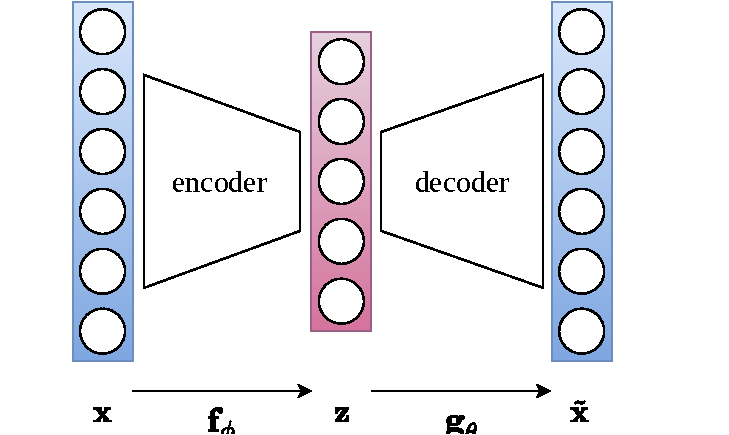
\includegraphics[height=4.5cm]{rc/autoencoder}
    \end{figure}

  \end{frame}

  \begin{frame}{Definition}

    \metroset{block=fill}

    \begin{alertblock}{Challenge}
      We do not want the encoder to learn the identity function, but to learn a \emph{good representation} of our data.
    \end{alertblock}

    \vspace{0.5cm}

    \begin{block}{Regularization?}
      Reducing the size of the \emph{hypothesis set} $\mathcal{H}$ by constraining the space of possible solutions to the optimization problem.
      \vspace{-0.25cm}
      \begin{itemize}
        \item L2 weight decay
        \item Sparsity, L1 weight decay
        \item \dots
      \end{itemize}
    \end{block}
    
  \end{frame}

  %
  \subsection{Mathematical formulation}
  %

  \begin{frame}{What is a good representation?}

    \metroset{block=fill}
    
    \small{Let $q_{\boldsymbol{\phi}}(Z|X)$ be a (stochastic) parametric mapping from $X$ to $Z$. A good representation $Z$ of a random variable $X$ maximizes \alert{mutual information} between $X$ and $Z$ (\emph{infomax principle}):}
    \vspace{0cm}
    \begin{align*}
      \mathbb{I}(X;Z) &= \mathbb{H}(X) - \mathbb{H}(X|Z)\\
                      &= C(X) + \mathbb{E}_{q_{\boldsymbol{\phi}}(X,Z)}\left[\log q_{\boldsymbol{\phi}}(X|Z)\right]
    \end{align*}

    \small{For any parametric distribution $p_{\boldsymbol{\theta}}(X|Z)$ we have $\mathbb{E}_{q_{\boldsymbol{\phi}}(X,Z)}\left[\log p_{\boldsymbol{\theta}}(X|Z)\right] \leq \mathbb{E}_{q_{\boldsymbol{\phi}}(X,Z)}\left[\log q_{\boldsymbol{\phi}}(X|Z)\right]$ (using $D_{KL}(q||p) \geq 0$).}

    \begin{block}{Task: maximize a lower bound on $\mathbb{I}(X;Z)$}
      \begin{equation*}
        \underset{\boldsymbol{\phi},\boldsymbol{\theta}}{\text{maximize}} \; \mathbb{E}_{q_{\boldsymbol{\phi}}(X,Z)}\left[\log p_{\boldsymbol{\theta}}(X|Z)\right]
      \end{equation*}
    \end{block}

  \end{frame}

  \begin{frame}{Loss function for deterministic autoencoders}

    We consider \alert{deterministic} mappings $Z = \mathbf{f}_{\boldsymbol{\phi}}(X)$ (or $q_{\boldsymbol{\phi}}(Z|X) = \delta(Z - \mathbf{f}_{\boldsymbol{\phi}}(X))$) and $\tilde{X} = \mathbf{g}_{\boldsymbol{\theta}}(\mathbf{f}_{\boldsymbol{\phi}}(X))$.
    \vspace{0cm}
    \begin{equation*}
      \underset{\boldsymbol{\phi},\boldsymbol{\theta}}{\text{maximize}} \; \mathbb{E}_{q_{\boldsymbol{\phi}}(X)}\left[\log p_{\boldsymbol{\theta}}(X|Z = \mathbf{f}_{\boldsymbol{\phi}}(X))\right]
    \end{equation*}

    Using empirical mean over a set of i.i.d. data samples:
    \vspace{0cm}
    \begin{equation*}
      \underset{\boldsymbol{\phi},\boldsymbol{\theta}}{\text{maximize}} \; \sum_i \log p_{\boldsymbol{\theta}}(\mathbf{x}^{(i)}|\mathbf{z}^{(i)} = \mathbf{f}_{\boldsymbol{\phi}}(\mathbf{x}^{(i)}))
    \end{equation*}

    equivalent to:
    \vspace{0cm}
    \begin{equation*}
      \underset{\boldsymbol{\phi},\boldsymbol{\theta}}{\text{maximize}} \; \sum_i \log p(\mathbf{x}^{(i)}|\tilde{\mathbf{x}}^{(i)} = \mathbf{g}_{\boldsymbol{\theta}}(\mathbf{f}_{\boldsymbol{\phi}}(\mathbf{x}^{(i)})))
    \end{equation*}

    Let us turn this into a minimization the negative sum of individual loss functions $\mathcal{L}(\mathbf{x}|\tilde{\mathbf{x}}) = -\log p(\mathbf{x}|\tilde{\mathbf{x}})$.
    
  \end{frame}

  \begin{frame}{Loss function for deterministic autoencoders}

    \metroset{block=fill}

    The reconstruction $\tilde{\mathbf{x}}$ is the \alert{mean} of a distribution that may have generated $\mathbf{x}$.

    \begin{block}{Continuous variables: $\mathbf{x} \in \mathbb{R}^d$}
      \begin{itemize}
        \item Gaussian distribution: $X|\tilde{X} = \tilde{\mathbf{x}} \sim \mathcal{N}(\tilde{\mathbf{x}}, \mathbf{\sigma}^2 \mathbf{I})$
      \item Loss function: $\mathcal{L}(\mathbf{x}|\tilde{\mathbf{x}}) \propto ||\mathbf{x} - \tilde{\mathbf{x}}||_2^2$      
      \end{itemize}
      $\rightarrow$ \alert{Mean Squared Error (MSE) loss}
    \end{block}

    \begin{block}{Binary variables: $\mathbf{x} \in \{0,1\}^d$, or $\mathbf{x} \in [0,1]^d$}
      \begin{itemize}
        \item Bernoulli distribution: $X|\tilde{X} = \tilde{\mathbf{x}} \sim \mathcal{B}(\tilde{\mathbf{x}})$
        \item Loss function: $-\sum_{j=1}^d [\mathbf{x}_j \log \tilde{\mathbf{x}}_j + (1-\mathbf{x}_j) \log (1-\tilde{\mathbf{x}}_j)]$
      \end{itemize}
      $\rightarrow$ \alert{Cross-entropy loss}
    \end{block}
    
  \end{frame}

  %%%
  \section{Neurons can learn principal components}
  %%%

  \begin{frame}{Hebb's Learning Rule}

  \end{frame}

  \begin{frame}{Learning PC with Oja's rule}

    \cite{Becker1991}, \cite{Oja1982}, \cite{Oja1992}
    
  \end{frame}

  %%%
  \section{Linear autoencoders}
  %%%

  \begin{frame}{Definition}

    \begin{figure}
      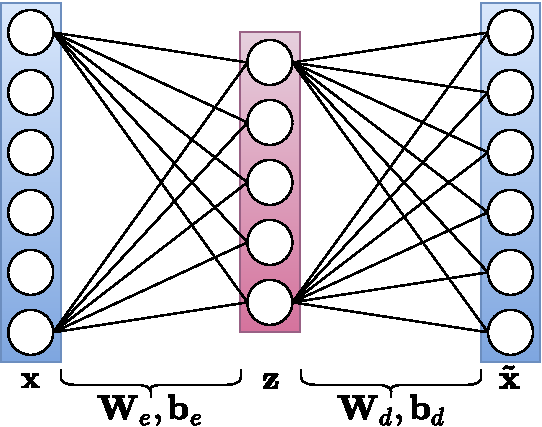
\includegraphics[width=7cm]{rc/linear-autoencoder}
    \end{figure}
    
  \end{frame}

  \begin{frame}{Similarity with PCA}

    Show equivalence to PCA

    \cite{Plaut2018}
    
  \end{frame}

  %%%
  \section{Non-linear autoencoders}
  %%%

  %
  \subsection{Non-linear and deep autoencoders}
  %

  \begin{frame}{Non-linear autoencoders}

    Non-linearity: sigmoid, tanh, ReLU\dots

    Several layers

    Not equivalent to PCA! (see paper AA-PCA)

  \end{frame}

  \begin{frame}{Deep autoencoders}

    Layer-wise pretraining: \cite{Hinton2006}
    In fact, not necessary (source?).
    
  \end{frame}

  %
  \subsection{Different types of regularization}
  %

  \begin{frame}{Undercomplete or overcomplete}
    
  \end{frame}

  \begin{frame}{Let's code! (1)}

    % AE classique avec une/plusieurs couches
    % Entraîner sur MNIST avec différents loss (MSE, cross-entropy)
    % Éventuellement convolutif

    % Observer l'espace latent via t-SNE (comparer avec t-SNE sur MNIST brut)
    
  \end{frame}

  \begin{frame}{The danger of overfitting}
    
    Problem: even a single continuous latent variable can remember the entire training set (one real number per sample).

    The latent space is not continuous.

  \end{frame}

  \begin{frame}{Sparse autoencoders}
    
  \end{frame}

  \begin{frame}{Denoising autoencoders}

    \cite{Vincent2010}
    
  \end{frame}

  %
  \subsection{Variational autoencoders (VAE)}
  %

  \begin{frame}{Motivations}
    
    Limitation of standard AE: the latent space has \emph{no structure} and may not be continuous; we cannot explore it nor sample from it.

    \begin{columns}[T,onlytextwidth]
      \column{0.5\textwidth}
      \centering
      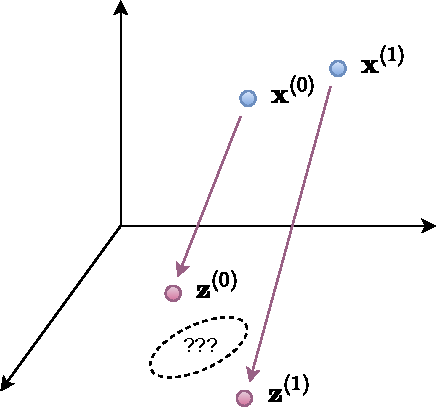
\includegraphics[width=0.8\textwidth]{rc/ae-latent}

      \column{0.5\textwidth}
      \centering
      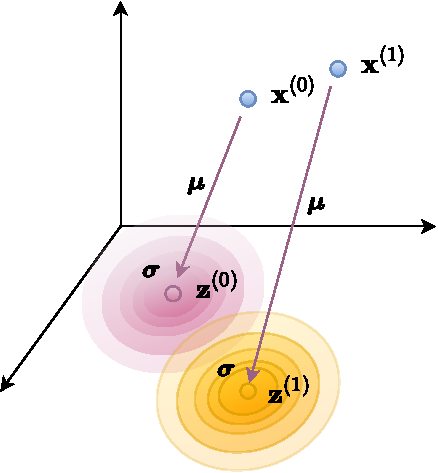
\includegraphics[width=0.8\textwidth]{rc/vae-latent}
    \end{columns}

    Example latent space figures, examples with MNIST, faces, music styles...

  \end{frame}

  \begin{frame}{Variational autoencoders (VAE)}
    
    \begin{columns}[T,onlytextwidth]

      \column{0.7\textwidth}
      \begin{block}{Probabilistic setting}
        \small{
        Generative model $p_{\boldsymbol{\theta}}(\mathbf{x}, \mathbf{z})$:
        \begin{enumerate}
          \item $\mathbf{z}$ sampled from $p_{\boldsymbol{\theta}}(\mathbf{z})$ (prior)
          \item $p_{\boldsymbol{\theta}}(\mathbf{x}|\mathbf{z})$ (likelihood/\emph{probabilistic decoder})
        \end{enumerate}
        Recognition model:\\
        $q_{\boldsymbol{\phi}}(\mathbf{z}|\mathbf{x})$ (approximate posterior/\emph{probabilistic encoder})
        }
      \end{block}

      \column{0.3\textwidth}
      \includegraphics[width=\textwidth]{rc/vae-gen}
      
    \end{columns}
    
    Stochastic gradient variational Bayes (SGVB) \cite{Kingma2014} is an efficient method to estimate the parameters in case of intractable likelihood/posterior and large datasets (as in DL).

    % Lien vers le blog VAE, utiliser des images

  \end{frame}

  \begin{frame}{VAE: the reparameterization trick}

    \begin{figure}
      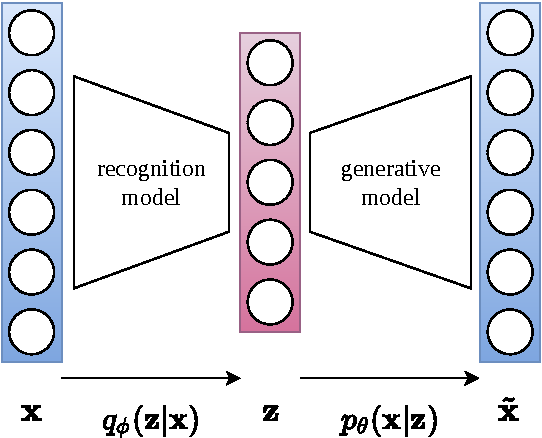
\includegraphics[width=7cm]{rc/vae}
    \end{figure}

  \end{frame}

  \begin{frame}{VAE loss function}

    \metroset{block=fill}
    
    \begin{exampleblock}{VAE ELBO (evidence lower bound)}
      \vspace{-0.25cm}
      \begin{equation*}
        \underset{\boldsymbol{\phi},\boldsymbol{\theta}}{\text{maximize}} \; -D_{KL}\left(q_{\boldsymbol{\phi}}(Z|X)||p_{\boldsymbol{\theta}}(Z)\right) + \mathbb{E}_{q_{\boldsymbol{\phi}}(Z|X)}\left[\log p_{\boldsymbol{\theta}}(X|Z)\right]
      \end{equation*}
    \end{exampleblock}

    \begin{alertblock}{Key ideas}
      \begin{itemize}
        \item The second term is a (negative) \alert{reconstruction error} (e.g. MSE or cross-entropy) as in a deterministic AE.
        \item The first term, a Kullback-Leibler divergence between $q_{\boldsymbol{\phi}}(Z|X)$ and $p_{\boldsymbol{\theta}}(Z)$, acts as a \alert{regularizer} pushing the encoder distribution closer to the prior distribution (typically a gaussian)
      \end{itemize}
    \end{alertblock}

  \end{frame}

  \begin{frame}{VAE loss function}

    \metroset{block=fill}
  
    Let's put gaussians everywhere!
    \begin{itemize}
      \item $p_{\boldsymbol{\theta}}(\mathbf{z}) = \mathcal{N}(\mathbf{z}; \mathbf{0}, \mathbf{I})$
      \item $q_{\boldsymbol{\phi}}(\mathbf{z}|\mathbf{x}) = \mathcal{N}(\mathbf{z}; \boldsymbol{\mu}, \boldsymbol{\sigma}^2\mathbf{I})$
    \end{itemize}

    \begin{block}{The reparameterization trick}
      To sample from $q_{\boldsymbol{\phi}}(\mathbf{z}|\mathbf{x})$, we use the reparameterization $\mathbf{z} = f_{\boldsymbol{\phi}}(\mathbf{x}, \epsilon) = \boldsymbol{\mu} + \boldsymbol{\sigma} \cdot \boldsymbol{\epsilon}$ where $\boldsymbol{\epsilon} \sim \mathcal{N}(\mathbf{0}, \mathbf{I})$
    \end{block}

    \small{For a given $\mathbf{x}^{(i)}$, and using 1-sample Monte-Carlo estimation, the ELBO becomes:}
    \vspace{0cm}
    \begin{multline*}
      \frac{1}{2} \sum_j \left(1 + \log (\boldsymbol{\sigma}^{(i)}_j)^2 - \boldsymbol{\mu}^{(i)}_j - (\boldsymbol{\sigma}^{(i)}_j)^2 \right) + \log p_{\boldsymbol{\theta}}(\mathbf{x}^{(i)}|\mathbf{z}^{(i)})\\
      \text{ where } \mathbf{z}^{(i)} = \boldsymbol{\mu}^{(i)} + \boldsymbol{\sigma}^{(i)} \cdot \boldsymbol{\epsilon}
    \end{multline*}

  \end{frame}

  \begin{frame}{VAE: the reparameterization trick}

    \begin{figure}
      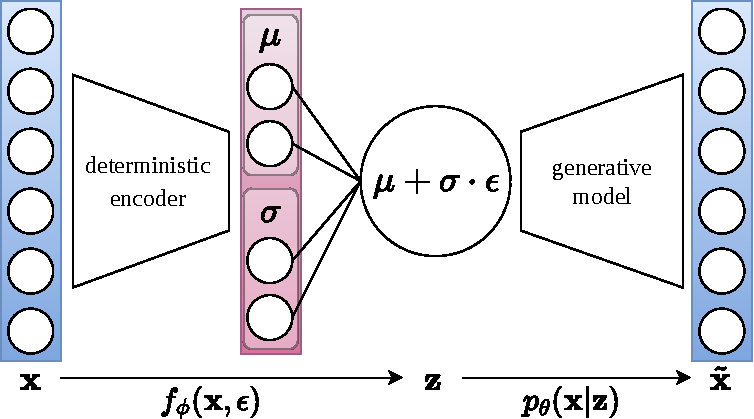
\includegraphics[width=9cm]{rc/vae-reparameterization}
    \end{figure}
    
  \end{frame}

  \begin{frame}{Let's code! (2)}

    % VAE avec une/plusieurs couches
    % Entraîner sur MNIST avec différents loss (MSE, cross-entropy)
    % Éventuellement convolutif

    % Observer l'espace latent via t-SNE (comparer avec AE)
    
  \end{frame}

  %%%
  \section{Applications}
  %%%

  \begin{frame}{Feature extraction}

    Dimensionality reduction, useful features

    Pre-processing pour d'autres algos (regress, classif, clustering)
    
  \end{frame}

  \begin{frame}{Unsupervised pretraining for supervised learning}
    
    Unsupervised pretraining -> supervised finetuning

    \cite{Erhan2010}

  \end{frame}

  \begin{frame}{Visualization}
    
  \end{frame}

  \begin{frame}{Data compression}
    
    Dimensionality reduction
    Data-specific, lossy compression.

  \end{frame}  

  \begin{frame}{Data augmentation}

    The decoder model can be used to \alert{generate new data samples}:

    \begin{itemize}
      \item Deterministic AEs: adding noise, interpolating or extrapolating in latent space \cite{Devries2017}
      \item Generative models (VAE, GAN)
    \end{itemize}

  \end{frame}

  \begin{frame}{Anomaly detection}
    
    When the input is different from the training data distribution (e.g. an outlier), the autoencoder will produce a large reconstruction error. This error can be used to \alert{score anomalies} \cite{Malhotra2016}.

    \begin{figure}
      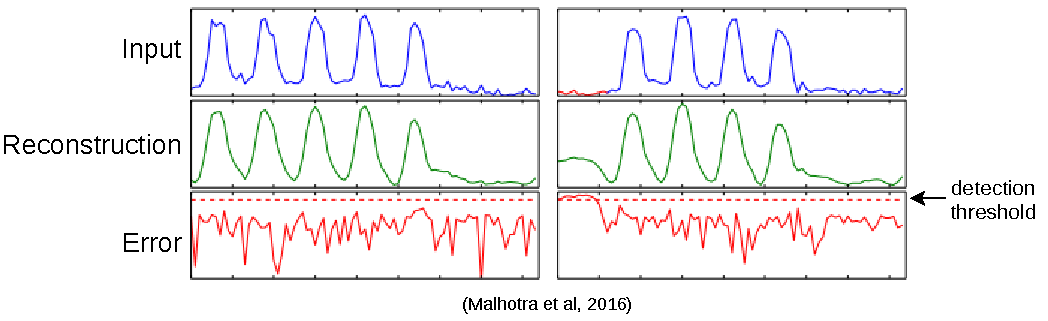
\includegraphics[width=10cm]{rc/anomaly-detection}
    \end{figure}

  \end{frame}

  %%%
  \appendix

  \begin{frame}[allowframebreaks]{References}
    
    \bibliography{references}
    \bibliographystyle{abbrv}
  
  \end{frame}

\end{document}